\section{مقدمه}
{
	اگرچه یادگیری ماشین سنتی در سال‌های اخیر به موفقیت‌های بزرگی دست یافته و در بسیاری از برنامه‌های کاربردی با موفقیت مورد استفاده قرار گرفته‌است، اما هنوز هم برای برخی از مسائل دنیای واقعی محدودیت‌هایی دارد. سناریوی ایده آل برای یادگیری ماشین این است که تعداد زیادی داده‌های آموزشی دارای برچسب وجود داشته باشد به طوری‌که توزیعی مشابه داده‌های تست  را داشته باشد. با این حال، جمع‌آوری داده‌های آموزشی کافی در بسیاری از سناریوها بسیار گران قیمت، وقت گیر یا حتی غیرممکن است. یادگیری نیمه نظارتی
	\footnote{\lr{Semi-supervised Learning}}
	 می‌تواند تا حدودی این مشکل را حل کند. رویکرد نیمه نظارتی فقط به تعداد محدودی از داده‌های برچسب‌‌‌خورده نیاز دارد و از مقدار زیادی از داده‌های بدون برچسب برای بهبود دقت یادگیری استفاده می‌کند. اما در بسیاری از موارد، جمع‌آوری نمونه‌های بدون برچسب نیز دشوار است.
	\cite{zhuang2020comprehensive}
	
	
	انتقال یادگیری
	\footnote{\lr{Transfer Learning}}
	، یک روش یادگیری ماشین برای حل مسئله فوق است. مفهوم انتقال یادگیری در ابتدا از روانشناسی ناشی شده است. طبق تئوری انتقال، انتقال یادگیری نتیجه عمومی شدن تجربه است. به  این معنی که کسی که ویولن را یاد گرفته است می‌تواند پیانو را سریعتر از دیگران بیاموزد، زیرا ویولن و پیانو سازهای موسیقی هستند و ممکن است دانش مشترکی با هم داشته باشند. شکل
	\ref{fig:9}
	چند مثال شهودی درباره انتقال یادگیری را نشان می‌دهد.
	
	 با الهام از توانایی‌های بشر برای انتقال دانش، انتقال یادگیری در یادگیری ماشین به این مفهوم است که دانش از یک حوزه مرتبط (به نام دامنه مبدا) برای بهبود عملکرد یادگیری در دامنه هدف منتقل می‌شود. گفتنی است، دانش منتقل شده همیشه تأثیر مثبتی در کارهای جدید نمی‌گذارد. اگر بین حوزه‌ها اشتراکی وجود داشته باشد، انتقال دانش می‌تواند ناموفق باشد. به عنوان مثال، یادگیری دوچرخه سواری نمی‌تواند به ما کمک کند سریعتر پیانو را یاد بگیریم. علاوه بر این، شباهت‌ها بین دامنه‌ها همیشه یادگیری را تسهیل نمی‌کند، زیرا گاهی اوقات شباهت‌ها ممکن است گمراه کننده باشد. به عنوان مثال‌، اگرچه اسپانیایی و فرانسوی رابطه نزدیکی با یکدیگر دارند، افرادی که اسپانیایی را یاد می‌گیرند ممکن است در یادگیری زبان فرانسه مشکلاتی از قبیل استفاده از واژگان اشتباه یا ترکیبات را تجربه کنند. این امر به این دلیل رخ می دهد که تجربه موفق قبلی در اسپانیایی می‌تواند در یادگیری کلمه، استفاده، تلفظ، ترکیب و غیره به زبان فرانسه اختلال ایجاد کند. در زمینه روانشناسی، این پدیده که تجربه قبلی در یادگیری کارهای جدید تأثیر منفی دارد، انتقال منفی نامیده می‌شود. به همین ترتیب، در حوزه انتقال یادگیری، اگر یادگیرنده هدف، تحت تأثیر منفی دانش منتقل شده باشد، به عنوان انتقال منفی نامیده می‌شود. این که آیا انتقال منفی اتفاق می‌افتد ممکن است به عوامل مختلفی بستگی داشته باشد از جمله ارتباط بین دامنه مبدا و هدف و ظرفیت یادگیرنده.
	\cite{zhuang2020comprehensive}
	\begin{figure}
		\centering
		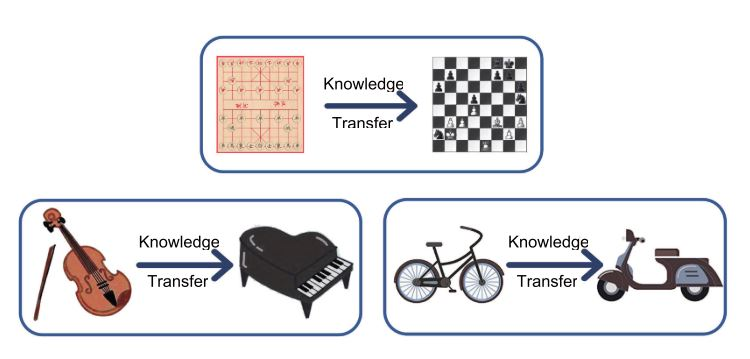
\includegraphics[scale=0.4]{images/example.jpg}
		\caption{مثالی از انتقال یادگیری \cite{zhuang2020comprehensive}}
		\label{fig:9}
	\end{figure}

	اصطلاح دیگری که معمولاً در انتقال یادگیری استفاده می‌شود تطبیق دامنه
	 \footnote{\lr{Domain Adaptation}}
	 است. تطبیق دامنه به فرایندی گفته می‌شود که یک یا چند دامنه مبدا برای انتقال دانش و بهبود عملکرد دامنه هدف تطببق داده می‌شوند. انتقال یادگیری غالباً به فرآیند تطبیق دامنه متکی است که سعی در کاهش تفاوت بین دامنه‌ها دارد.
	 \cite{weiss2016survey}
	
}